\section{Введение}
В начале XIX века люди испытывали трудности со временем -- не в том, сколько 
его у них было, а в том, чтобы знать, который сейчас час. Часы, конечно же, 
уже были придуманы, но в каждом городе было свое время, <<местное время>>, 
которое синхронизировалось между часовыми башнями города, чаще всего с 
помощью церковного звона. Позже <<Время Железной Дороги>> (Railway Time), а 
затем и Среднее Время по Гринвичу (GMT) постепенно заменили собой все 
<<местное время>>, и большинство людей сегодня даже не представляют себе, что 
время -- это не некая универсальная вещь.

<<Проблема времени>> сегодня -- это география, и все ищут эталонный источник. 
Google ежегодно тратит около 1 миллиарда долларов, поддерживая свои карты в 
актуальном состоянии, и, помимо этого, Google потратила 1.5 миллиарда,
купив Waze\cite{waze}. И Google далеко не единственная компания,
которая пытается купить все, что только можно, связанное с картами, ибо 
Nokia купила Navteq\cite{navteq}, а TomTom\cite{tomtom} и 
Tele Atlas\cite{teleatlas} работают над слиянием. Все эти компании пытаются 
стать тем самым эталонным источником информации о том, что находится на земле.

Но раз существуют все эти компании, то для чего же нужен такой проект как 
OpenStreetMap? Ответ лежит в простой идее о том, что ни одна компания не 
должна обладать монополией на <<место>>, точно так же как ни одна компания не 
обладала монополией на <<время>> в начале XIX века. <<Место>> является общим 
ресурсом, и если вы дадите всю власть над ним одной компании, вы дадите ей 
власть не только сообщать о том, где вы находитесь, но и силу искажать эту 
информацию. Проще говоря, есть три пункта: кто решает, что показывать на 
карте; кто решает где вы находитесь и куда направляетесь; а также вопрос 
личной приватности.

Все эти поставщики карт заинтересованы в том, чтобы собирать информацию о вас, 
включая способы, с которыми вы вполне можете быть не согласны. Как Google, так 
и Apple собирают информацию о вашем местоположении, когда вы пользуетесь их 
сервисами. Они используют эту информацию, чтобы улучшить точность карт, но 
Google уже объявила, что собирается определять зависимость между тем, что вы 
ищете и тем, куда направляетесь. С 500 миллионами телефонов на Android это 
гигантский объем информации о том, какие привычки отдельно взятых людей 
проявляются когда они просто гуляют, когда едут на работу, идут в больницу, а 
то и принимают участие в акции протеста. Однозначно, нельзя игнорировать 
влияние на общество того факта, что вся эта куча данных находится в одних 
руках, сколь бы благородными они не представлялись. Компании вроде 
Foursquare\cite{four4} используют игровой процесс, чтобы скрыть то, что по 
сути является процессом сбора огромного количества данных, и даже Google уже 
включилась в эту игру с геймификацией в Ingress\cite{ingress} -- игрой, 
которая накладывает искусственный мир поверх нашего реального и поощряет 
пользователей собирать информацию о маршрутах и делать фотографии в
игровом процессе.

Касательно содержимого карт, OpenStreetMap является и нейтральной и 
прозрачной. OpenStreetMap является подобной Вики картой, которую может 
редактировать кто угодно. Если магазин отсутствует на карте, его может 
добавить как владелец магазина, так и его посетитель. Что касается показа 
(рендеринга) карты, то любой человек или компания, принимающие участие в 
создании карты, свободен рендерить ее как ему удобно. Главная карта на 
\url{OpenStreetMap.org} использует ПО рендеринга и стиль со свободной 
лицензией, которые кто угодно может взять и подправить под свои нужды. 
Проще говоря, любой, кому необходимо, всегда может создать свои собственные 
карты, основываясь на данных OSM.

Также, несмотря на то, что самые популярные построители маршрутов для 
OpenStreetMap лицензированы под FLOSS\cite{floss}, даже если какая-нибудь 
компания и выберет другую лицензию, пользователи всегда могут использовать 
свои построители маршрутов, и сравнив результаты построения, выявить 
какие-либо подтасовки, если они есть.

И наконец, пользователь волен скачать любую часть или даже всю карту 
OpenStreetMap для использования в оффлайне. Это означает, что можно 
использовать данные OpenStreetMap для навигации, вообще не передавая 
информацию о вашем местоположении на сторону.\cite{habrahabr01}

\section{OpenStreetMap}
\subsection{Общие сведения}
OpenStreetMap -- некоммерческий веб-картографический проект, который создает и 
предоставляет свободные географические данные и возможность создавать карты 
всего мира кому угодно, кто это хочет. Авторы начали этот проект, потому что 
большинство карт, о которых вы думаете, что они свободны, на самом деле имеют 
юридические или технические ограничения на их использование, сдерживают людей 
от их использования творческим, эффективным или неожиданным образами. 

Проект предоставляет карту всего мира, которую может редактировать каждый, 
которая создается практически с чистого листа по GPS-трекам и распространяется 
под свободной лицензией.

Лицензия OpenStreetMap позволяет свободно (или почти свободно) получать доступ 
ко всем растровым картам и всем лежащим в их основе пространственным 
данным, и этот проект направлен на поощрение нового и интересного 
использования этих данных.\cite{osmwiki}

\subsection{История возникновения и развития}
Стив Кост был вдохновлен успехом Википедии и решил, что принцип вики, 
заложенный в основу Википедии, может применяться и для веб-картографии. Для 
реализации своих идей в Великобритании в июле 2004 года он создал проект 
OpenStreetMap. Это произошло еще до появления Google Maps, и цель 
OpenStreetMap -- получить бесплатную карту мира, опираясь на добровольцев с 
GPS-устройствами, казалась трудноосуществимой. Единственным образцом для 
подражания в подобном массовом добровольном сборе данных была Википедия, 
которая к тому времени уже была серьезным конкурентом коммерческих 
энциклопедий.

В январе 2007 года Кембридж стал первым полностью отрисованным городом, и к 
июлю 2007 года, когда состоялась первая международная конференция OSM под 
названием The State of the Map, в проекте на то время было 9000 
зарегистрированных участников. Спонсорами мероприятия были в том числе Google, 
Yahoo и Multimap.

В январе 2008 была реализована возможность загрузки картографических данных в 
GPS-устройство для использования велосипедистами. В марте двое основателей
анонсировали, что они получили венчурный капитал в 2.4 млн евро для CloudMade,
коммерческой компании, которая будет использовать данные OpenStreetMap.
4 марта 2008 года создан русскоязычный раздел на форуме, ставший самым
популярным разделом на форуме OSM.

В январе, когда случилось катастрофическое землетрясение на Гаити, тысячи 
участников проекта приняли участие в составлении и актуализации карты Гаити. 
Это подняло популярность OpenStreetMap: был введен в широкое использование 
термин <<crisis mapping>>, многие СМИ написали о проекте. Для использования в 
OSM свои спутниковые снимки предоставили NOAA, GeoEye, DigitalGlobe, ErosB, 
CNES / Spot Image, JAXA/ALOS, Google, WorldBank, в навигаторах данные с картой 
Гаити стали использовать американские спасатели.

После того как произошли разрушительные землетрясение и цунами в Японии и 
огромное количество домов просто смыло, участники OSM вне Японии по полученным 
свежим спутниковым снимкам (DigitalGlobe, JAXA/ALOS, MapQuest Open Aerial, 
Bing, Cnes / SpotImage, Aerial orthophotos from Japanese mapping authority 
GSI) стали отмечать последствия катастрофы, а сами японцы на местах -- 
источники воды, работающие магазины, телефоны и прочее.\cite{osmwiki}

\subsection{Возможности платформы}
Проект OpenStreetMap обладает большими функциональными возможностями. От 
свободных картографических данных, до разработки программного обеспечения на 
основе OSM. Стоит отметить большое количество, которые были разработаны на 
основе или с использованием OpenStreetMap. Среди них: картографические 
системы, навигационные системы, системы редактирования картографических данных 
и многие другие.\cite{osmwiki}

Выделим главные особенности платформы:
\begin{itemize}
    \item Проект охватывает всю поверхность земного шара.
    \item Главной целью проекта является построение не собственно карты, а 
        базы данных, содержащей сведения о точках на земной поверхности. Таким 
        образом, на основе собранных в рамках проекта данных можно создавать 
        карты различного вида и другие сервисы.
    \item Карты OpenStreetMap двумерные, без отображения высот над уровнем 
        моря, изолиний. Однако существуют проекты, которые отображают 
        рельефные карты, используя данные о высотах из сторонних свободных 
        источников.
    \item Возможен экспорт карт в форматы PNG, JPEG, SVG, PDF, PostScript. 
        Также существуют проекты по экспорту данных OpenStreetMap в форматы 
        Garmin и ГисРусса.
\end{itemize}

\subsection{Формат данных}
Значительный объем данных, загружаемых в OSM, выгружается из переносных 
устройств спутниковой навигации или мониторинга. Для конвертации координат 
из <<сырого>> (NMEA) или проприетарных форматов в формат GPX (основан на XML) 
может использоваться программа GPSBabel. Данные, собранные в формате WGS84 в 
виде широты/долготы, обычно показываются в проекции Меркатора\cite{projection}.

В целом, всю структуру данных можно представить схематично на следующем рисунке:
\begin{figure}[ht!]
    \center
    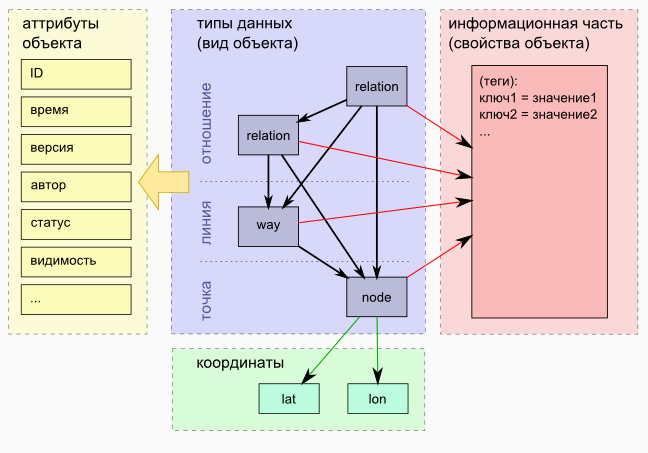
\includegraphics[width=0.47\textwidth]{p1}
    \caption{Структура данных OpenStreetMap.}
\end{figure}

Все данные можно условно разбить на три основные группы:
\begin{itemize}
    \item типы данных, описывающие в виде иерархической связи сам объект, как 
        некую пространственную сущность, имеющую свой конечный результат -- 
        известные координаты всех частей объекта;
    \item информационная часть -- это описательная характеристика объекта, не 
        имеющая к пространственной географической структуре объекта прямого 
        отношения (его название, физические, логические и прочие свойства);
    \item служебные атрибуты объекта, необходимые для организации процесса 
        хранения и обработки информации в виде набора данных, такие как 
        уникальный идентификатор, состояние объекта в базе, время последней 
        правки объекта в базе и т.д.
\end{itemize}

\subsubsection{Базовые типы географических данных в OpenStreetMap}
\label{part01}
Базовых типов по сути всего три: точка (\emph{node}), линия (\emph{way}) и 
отношение (\emph{relation}). Сами типы \emph{node}, \emph{way} и 
\emph{relation} называются так, потому что именно так они были придуманы 
изначально. Все без исключения объекты в OSM описываются этими тремя типами 
данных, после чего информационно наполняются комбинациями тегов. Модель данных 
в OSM строится на иерархической ссылочной структуре, из чего следует, что 
любой последующий тип данных не содержит информацию содержащуюся в предыдущих 
типах а образует новую сущность, ссылаясь на некое множество объектов 
предыдущего типа. Так же следует упомянуть, что любой объект имеет в структуре 
данных OSM свой идентификатор (\emph{ID}), уникальный в пределах данного типа 
объектов. Именно по этому идентификатору и происходит ссылка на сам объект. 
Рассмотрим структуру базовых типов по порядку.

\textbf{Первый тип: точка (\emph{node})} -- это минимальный набор данных, 
который содержит в себе информацию о паре координат: широта, долгота 
(\emph{lat}, \emph{lon}) и является базовым в иерархической модели. Это 
единственный тип данных, который хранит саму географическую информацию -- 
координаты, в виде широты и долготы. Модель данных OSM оперирует исключительно 
двухмерными данными в пределах проекции WGS84. В дальнейшем мы будем считать, 
что координаты -- это не информационная составляющая объекта точки, а 
неотъемлемая часть его структуры. В XML нотации, объект данного типа будет 
выглядеть так:

\small
\begin{verbatim}
<node id='19' lat='58.888047127548994' lon='49.747870758186764' />
\end{verbatim}
\normalsize

Одна точка с уникальным \emph{id} равным 19 и парой координат. Координаты в 
OSM используются в десятичной записи, поскольку это гораздо проще обрабатывать 
чем форматы координат с минутами и секундами. Сама по себе точка может быть 
самостоятельным объектом, описывающим какой-то точечный объект (геометрический 
примитив) или не иметь вовсе собственной информационной составляющей, а быть 
частью другого объекта (линии или отношения). При этом, забегая немного 
вперед, отметим, что точка одновременно может быть и самостоятельным объектом, 
несущим уникальную информацию и быть частью другого объекта.

\textbf{Второй тип данных: линия (\emph{way})} -- это совокупность указателей 
на объекты типа точка (\emph{node}). Как минимум, линия состоит из одной 
точки, т.~е. должна содержать как минимум одну ссылку на уже существующий 
объект типа точка. Линия из одной точки не противоречит структуре данных OSM, 
но противоречит понятиям элементарной геометрии, поэтому правильная линия
всегда содержит как минимум ссылки на два существующих объекта типа точка.

Правильная XML нотация объекта типа линия будет заключаться в описании всех 
необходимых точек, после чего следует сама запись о линии, в которой 
перечисляются все ее точки. В простейшем варианте это будет выглядеть так:

\small
\begin{verbatim}
<node id='23' lat='58.875047918145675' lon='49.785240674006126' />
<node id='22' lat='58.86687448573524' lon='49.737090974777324' />

<way id='24'>
  <nd ref='22' />
  <nd ref='23' />
</way>
\end{verbatim}
\normalsize

Порядок перечисления точек в линии важен, он характеризует последовательность 
точек в линии и направление самой линии, т.~е. у линии всегда есть начало и 
конец, даже если она замкнутая (в этом случае они просто совпадают). В данном 
примере мы вначале описали две точки, задав их координаты, а потом описали 
линию, сославшись на id этих точек. Одна точка может входить в любое количество 
объектов линий, при этом должна быть описана только один раз, т.~е. точка может 
быть общей для двух линий, в этом случае ссылка на нее содержится в обоих 
линиях. Таким образом строится цельный граф объектов (чаще всего дорожный граф 
для расчета роутинга), который представляет из себя совокупность объектов 
(линий), имеющих связь через их общие члены (точки).

Если мы хотим создать еще одну линию из уже существующих точек 19 и 23, то мы 
опишем ее так:

\small
\begin{verbatim}
<way id='48'>
  <nd ref='19' />
  <nd ref='23' />
</way>
\end{verbatim}
\normalsize

В нашем случае точки 19 и 23 уже описаны выше, а точка 23 вошла в состав двух 
линий 24 и 48 и стала общей для них.

Наши линии 24 и 48 можно графически представить в проекции меркартора следующим 
образом:

\begin{figure}[ht!]
    \center
    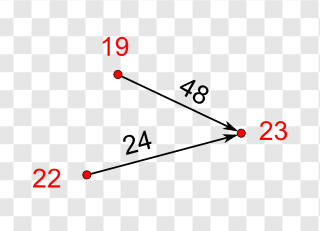
\includegraphics[width=0.47\textwidth]{p2}
    \caption{Две линии}
\end{figure}

Подписи на рисунке -- \emph{id} объектов: красные у точек, черные у линий; 
стрелкой указано направление линии, т.~е. обе линии заканчиваются на точке 23.

\textbf{Следующий тип данных: отношения (\emph{relation}).} По сути все 
объекты кроме точки -- уже отношения, однако линии выделены в отдельный тип 
данных как наиболее распространенные, описывающие основные геометрические 
примитивы: линии, полилинии и полигоны. Для всех более сложных геометрических 
объектов, а так же для объектов являющихся не чисто геометрическими, а 
логическими (коллекции, списки, иерархии взаимосвязей) предназначен 
универсальный тип данных -- отношения.

В целом, описание отношения отличается от линии тем, что линия -- это всегда 
совокупность точек, а отношение -- это совокупность любых объектов, как точек 
и линий, так и других отношений. Следовательно в отношениях указывается не 
только \emph{id} объекта, но и его тип. В самом минимальном варианте отношение 
может содержать ссылку только на один объект. Оперируя объектами описанными в 
примерах выше, можно написать отношение:

\small
\begin{verbatim}
<relation id='31'>
  <member type='way' ref='24' />
  <member type='node' ref='19' />
</relation>
\end{verbatim}
\normalsize

Это фиктивное абстрактное отношение, описывающее, что в него входит два 
объекта (члены отношения) -- точка 24 и линия 19 и более не несущее никакой 
другой информации. В реальном случае у отношения должен быть указан тип, как 
тег (информационная составляющая) самого объекта отношения, а у членов 
отношения должны быть указаны роли в ссылках на объекты.

Ниже приведен пример самого распространенного отношения типа <<мультиполигон>>, 
которое описывает один замкнутый внешний полигон из трех точек с вырезанным из 
него замкнутым полигоном тоже из трех точек меньшего размера. О геометрических 
примитивах (замкнутых и не замкнутых полигонах) и тегах объектов речь пойдет 
далее, а пока следует обратить внимание на параметры ролей (\emph{role}) у 
объектов отношения и наличие тега описывающего тип. 

\small
\begin{verbatim}
<node id='1218' lat='58.870941122729505' lon='49.758021019729554' />
<node id='1216' lat='58.8704000725183' lon='49.74703196841415' />
<node id='1215' lat='58.879055860772034' lon='49.74964840920353' />
<node id='1209' lat='58.86471853452049' lon='49.780522410518245' />
<node id='1207' lat='58.863365649894774' lon='49.72453057762546' />
<node id='1206' lat='58.892035483174' lon='49.74755525657201' />
<way id='1217'>
  <nd ref='1215' />
  <nd ref='1216' />
  <nd ref='1218' />
  <nd ref='1215' />
</way>
<way id='1208'>
  <nd ref='1206' />
  <nd ref='1207' />
  <nd ref='1209' />
  <nd ref='1206' />
</way>
<relation id='1221'>
  <member type='way' ref='1208' role='outer' />
  <member type='way' ref='1217' role='inner' />
  <tag k='type' v='multipolygon' />
</relation>
\end{verbatim}
\normalsize

Роль outer говорит о том, что данный объект будет наружным контуром 
графического объекта, а роль \emph{inner} сообщает о том, что пространство 
внутри этого объекта необходимо исключить из площади результирующего объекта. 
Графически наш мультиполигон будет выглядеть так:

\begin{figure}[ht!]
    \center
    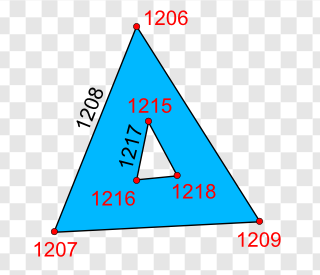
\includegraphics[width=0.47\textwidth]{p3}
    \caption{Мультиполигон}
    \label{multipoly01}
\end{figure}

Так же как и у линии, у отношения порядок перечисления членов играет роль и 
учитывается при использовании этого отношения. Например отношением может быть 
не геометрическая фигура, а маршрут общественного транспорта (логическая 
схема), тогда в него входят последовательно участки дорог, по которым будет 
двигаться автобус и список точек -- остановки на которых он останавливается, 
следовательно порядок включения дорог в отношение показывает последовательность 
прохождения маршрута, а порядок остановок -- последовательность их посещения.

Объект \emph{relation} может быть членом другого \emph{relation}, при этом 
уровень вложенности и иерархия вверх ничем не ограничивается. Структурное 
ограничение заключается в том, что объект \emph{relation} не может быть членом 
самого себя, т.~е. содержать ссылок на самого себя. Рекурсия в структуре типов 
данных в OSM недопустима, хотя конечно ничто не мешает создать такой объект 
и даже вполне успешно воткнуть его в базу данных.

Определив три базовых типа объектов надо ввести понятие начального и конечного 
объекта. Начальным объектом является любой объект, который входит в состав 
любого другого объекта, т.~е. является дочерним по отношению как минимум к 
одному объекту, но сам при этом ни включает ни одного другого объекта. В 
случае OSM это всегда точка. Либо другое его определение -- начальный объект 
несет в своей структуре (не в информационной части!) только географические 
координаты и не содержит ссылок на другие объекты.

Конечным объектом является максимальный по иерархии родительский объект, 
который не является дочерним по отношении ни к одному другому объекту, т.~е. не 
входит в состав ни одного другого объекта. Это может быть любой из трех 
перечисленных типов: точки, линии, отношения. Отдельный точечный объект, 
никуда не входящий, состоящий из одного объекта типа точка, не является 
начальным объектом, поскольку не является началом иерархии объектов, но 
является конечным объектом, поскольку на нем заканчивается пространственное 
описание объекта.\cite{habrahabr02}

\subsubsection{Информационная схема объектов}
Тип объекта описывает географические (пространственные) свойства объекта, но 
ничего не говорит о свойствах самого объекта, его характеристиках, назначении 
и прочем. Для это существует информационная часть структуры данных OSM, 
основанная на принципах тегирования объектов, т.~е. назначении им определенных 
меток и указанием свойств этих меток. Теги задаются в виде пары 
\emph{ключ} = \emph{значение}, что в нотации XML для нашей линии 24 выглядит 
так:

\small
\begin{verbatim}
<way id='24'>
  <nd ref='22' />
  <nd ref='23' />
  <tag k='highway' v='primary' />
</way>
\end{verbatim}
\normalsize

В данном случае мы добавили свойство нашей линии, а именно указали тег 
\emph{highway} со значением \emph{primary}, что в принятой схеме тегирования 
обозначает что наша линия является основной дорогой (дорога класса ниже 
магистрали, но выше второстепенной). Тегов у любого объекта может сколько 
угодно много, что позволяет задать все его основные свойства и описать все 
второстепенные параметры, а так же в произвольной форме дополнить объект любой 
информацией. Сама схема тегирования в OSM является одновременно самым главным 
ее архитектурным преимуществом, поскольку позволяет описать фактически любые 
свойства объекта, т.~к. реально никто не ограничивает вас в выборе новых тегов 
для новых свойств объектов; и одновременно самым больным ее местом, поскольку 
любая свобода в выборе способов обозначения всегда порождает религиозные войны 
различных групп пользователей, так и не сошедшихся во мнении, как обозначать 
тот или иной спорный объект.

Если мы немного расширим информационное описание наших двух линий 24 и 48 из 
первой части, то можем получить что-то вроде:

\small
\begin{verbatim}
<node id='23' lat='58.87753645355202' lon='49.79290110146539'>
  <tag k='highway' v='traffic_signals' />
</node>
<node id='22' lat='58.87456113991739' lon='49.73690926857261' />
<node id='19' lat='58.89362576054878' lon='49.7492065402827' />
<way id='48'>
  <nd ref='19' />
  <nd ref='23' />
  <tag k='embankment' v='yes' />
  <tag k='highway' v='secondary' />
  <tag k='incline' v='up' />
  <tag k='lanes' v='2' />
  <tag k='maxspeed' v='60' />
  <tag k='name' v='улица Пожарского' />
</way>
<way id='24'>
  <nd ref='22' />
  <nd ref='23' />
  <tag k='highway' v='primary' />
  <tag k='lanes' v='6' />
  <tag k='lit' v='yes' />
  <tag k='name' v='проспект Минина' />
  <tag k='oneway' v='yes' />
  <tag k='ref' v='М84' />
</way>
\end{verbatim}
\normalsize

Линия 48 у нас стала <<улицей Пожарского>>, с ограничением скорости в 
60 км/час, количеством полос равным двум, имеющей положительный градиент 
уклона в сторону от точки 19 к точке 23, являющейся второстепенной дорогой и 
поднятой относительно уровня земли на насыпь. А линия 24 у нас основная дорога 
(классом выше чем secondary) с 6-тю полосами движения, имеющей стационарное 
освещение и одностороннее движение разрешенное в направлении от точки 22 в 
сторону точки 23, носит название <<проспект Минина>> и является частью 
федеральной трассы М84. Обе дороги имеют общую точку 23, которая является 
перекрестком со светофором. \cite{habrahabr02}

\subsubsection{Геометрические примитивы}
Основная или как минимум наиболее частая задача для любых географических 
пространственных данных -- получение графического представления объектов, 
описанных этими данными. Проще говоря рендеринг самих карт, схем, планов. Сами 
алгоритмы, правила, стили и методы рендеринга карт -- это задача уже 
прикладного софта, но все сводится к отрисовке основных геометрических 
примитивов, которые получаются из объектов трех типов данных, перечисленных в 
\ref{part01}.

Итак, из чего формируются основные геометрические примитивы.

\textbf{Точка (\emph{point})} -- это один объект типа \emph{node}. Положению 
ее в заданной проекции на карте соответствует ее пространственное положение в 
географических координатах. Одна пара координат \emph{lat}/\emph{lon} 
транслируется в координаты x/y карты с учетом проекции.

\textbf{Линия (\emph{line})} -- это, как мы уже сказали, кратчайшее растояние 
между двумя точками, соответствует объекту типа \emph{way}, содержащему два 
объекта node. Любые два \emph{node}, поскольку мы оперируем плоским 
пространством, а следовательно расстояние между любыми двумя точками всегда 
будет прямой линией.

\textbf{Полилиния (\emph{polyline})} -- это связанная последовательность 
сегментов, где каждый сегмент представляет из себя одну линию, связанную своим 
концом с началом следующего сегмента. Вся последовательность является единым 
цельным объектом. Соответствует объекту \emph{way} содержащему три и более 
\emph{node}. Полилиния может быть объектом \emph{relation}, содержащим 
последовательно включенные объекты \emph{way}, где каждый следующий объект 
\emph{way} начинается с объекта \emph{node}, которым закончился предыдущий 
\emph{way}. Полилиния может быть либо объектом \emph{way}, содержащим 
\emph{node}, либо \emph{relation}, содержащим \emph{way}, т.~е. не может быть 
\emph{relation} содержащим и \emph{way} и \emph{node} одновременно, однако 
может быть объектом \emph{relation}, содержащим одновременно \emph{way} и 
другие \emph{relation}, содержащие только объекты \emph{way}.

Виды полилиний:

\begin{figure}[ht!]
    \center
    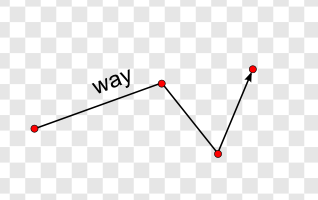
\includegraphics[width=0.47\textwidth]{p4}
    \caption{polyline = way(node1,node2,node3,node4)}
    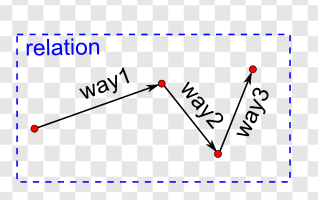
\includegraphics[width=0.47\textwidth]{p5}
    \caption{polyline = relation( way1(node1,node2), 
        way2(node2,node3), way3(node3,node4) )}
    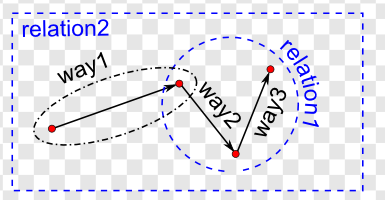
\includegraphics[width=0.47\textwidth]{p6}
    \caption{polyline = relation2( way1(node1,node2), 
        relation1( way2(node2,node3), way3(node3,node4) ) )}
\end{figure}

\textbf{Полигон (\emph{polygon})} -- это замкнутая полилиния, у которой 
последняя точка совпадает с первой. В типах данных OSM соответствует объекту 
\emph{way} с несколькими (три и более) объектами \emph{node}, при этом 
количество членов объекта \emph{way} всегда больше на единицу, т.~к. первый 
объект \emph{node} повторяется дважды: в начале и в конце списка. Так же 
полигон может быть собран в виде \emph{relation}, в который последовательно 
включаются \emph{way}, образующие совместно замкнутый контур, т.~е. началу 
каждого объекта \emph{way} соответствует конец одного другого объекта 
\emph{way}. В отличии от полигона в \emph{way}, полигон в \emph{relation} не 
дублирует последний объект в перечислении с первого, поскольку для \emph{way} 
это необходимо в связи с тем, что он ссылается на объекты \emph{node} и 
только по факту дублирования \emph{node} как первого и последнего элемента 
списка членов можно судить о том что это замкнутый полигон, а не линейный 
объект полилиния. В полигоне собранном в виде \emph{relation} последний объект 
\emph{node} последнего включенного объекта \emph{way} или \emph{relation} 
содержащего \emph{way} соответствует первому объекту node первого включенного 
\emph{way}.

В случае полигона описываемого в виде \emph{relation}, обязательно указывается 
тег \emph{type} = \emph{multipolygon} на самом объекте \emph{relation}. Таким 
образом мы определяем, что речь идет о площадном геометрическом, а не о 
линейном объекте.

Виды полигонов:

\begin{figure}[ht!]
    \center
    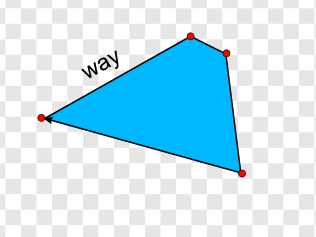
\includegraphics[width=0.47\textwidth]{p7}
    \caption{polygon = way(node1,node2,node3,node4,node1)}
    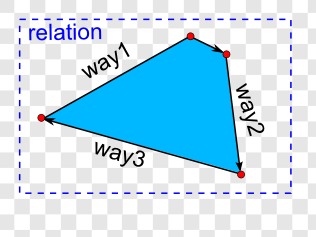
\includegraphics[width=0.47\textwidth]{p8}
    \caption{polygon = relation( way1(node1,node2,node3), 
        way2(node3,node4), way3(node4,node1) )}
    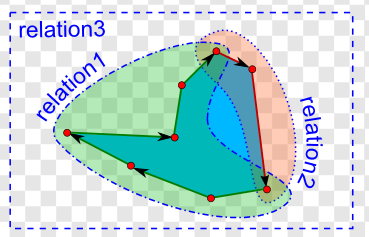
\includegraphics[width=0.47\textwidth]{p9}
    \caption{polygon = relation3( relation1( way1(node1,node2,node3), 
        way2(node3,node4), way3(node4,node5), 
        way4(node5,node6,node7) ), relation2( way5(node7,node8), 
        way6(node8,node1) ) )}
\end{figure}

Составные объекты -- это объекты которые невозможно описать одним примитивом 
\emph{way}, всегда строятся на базе объектов \emph{relation} у которого 
\emph{type}=\emph{multipolygon}. Полигоны и полилинии описанные в виде 
\emph{relation} всегда можно упростить до одного объекта \emph{way}, в то 
время как составной объект в самом упрощенном случае дает минимум два объекта 
\emph{way}. Например это площадная фигура (полигон) из которой математически 
вычтена другая фигура (полигон меньшего размера). Пример мультиполигона, 
являющегося составным объектом, с иллюстрацией был приведен на рисунке 
\ref{multipoly01}, в описании объектов \emph{relation}.

Мультиполигоны для составных объектов, так же как и полигоны и полилинии могут 
собираться из простых way или из других \emph{relation}, состоящих из любого 
количества \emph{way}. Для такого мультиполигона обязательно указание роли для 
каждого входящего члена, будь то \emph{way} или \emph{relation}. Как минимум 
должен быть один член с ролью \emph{outer}. Именно объект или объекты с этой 
ролью задают главный (внешний) геометрический контур результирующего объекта. 
Объектов с ролью \emph{inner} может и не быть в частном случае, но тогда такой 
мультиполигон -- это обычный полигон, просто описанный избыточно. Объекты с 
ролью \emph{inner} указывают какие участки, находящиеся внутри внешнего 
контура, не являются частью результирующей фигуры. Например это поляна в лесу 
или внутренний двор дома, ограниченный со всех сторон стенами этого дома.

Все объекты с одной ролью в одном мультиполигоне должны собраться в один или 
несколько замкнутых не пересекающихся по границам контуров.\cite{habrahabr01}

\section{Leaflet}
\subsection{Введение}

Leaflet является современный открытым проектом написанная на JavaScript 
библиотека для отображения мобильных интерактивных карт. Она разработана 
Владимиром Агафонкиным и командой. При весе всего около 33 КБ JS, он имеет все 
функции, которые могут понадобиться большинству разработчиков для отображения 
интернет-карт.

Leaflet задумана как библиотека, одинаково хорошо работающая и на десктопных 
браузерах, и на мобильных устройствах (iPhone/iPad, Android) -- очень быстрая, 
легковесная, с простым API, красивым и понятным ООП-кодом. В отличии от 
OpenLayers\cite{openlayers} авторы не пытаемся впихнуть в нее все фичи, о 
которых только можно помыслить, раздувая код до немыслимых размеров -- 
только самое основное, минимальный набор, который удовлетворяет нужды 99\% 
применений карт в онлайне (тайлы, маркеры, векторы, попапы), но 
реализовывая их максимально лучшим образом.

Библиотека Leaflet разработана с упором на простоту и производительность, а 
также для удобного использования где угодно. Она работает эффективно на всех 
основных настольных и мобильных платформ из коробки, пользуясь HTML5 и CSS3 
на современных браузерах. Функциональность библиотеки может быть расширена 
с помощью огромного количества плагинов, имеющие хорошо документированный и 
простой API, красивый и легко читаемый исходных код.\cite{leaflet}

\subsection{Возможности библиотеки}
Доступные слои:
\begin{itemize}
    \item Слой тайлов (<<плиток>> карты)
    \item Маркеры
    \item Всплывающие элементы
    \item Векторные элементы: линии, многоугольники (полигоны), круги,
        круглые маркеры
    \item GeoJSON слои
    \item Накладываемые изображения / слои
    \item Слой WMS
    \item Группы слоев
\end{itemize}

Поддержка браузеров:
\begin{itemize}
    \item Firefox 3.6+
    \item Chrome
    \item Safari 5+
    \item Opera 11.11+
    \item IE 7–9
    \item IE 6 (не отлично, но достаточно)
    \item Safari for iOS 3/4/5+
    \item WebKit for Android 2.2+, 3.1+, 4+
\end{itemize}

Все доступные возможности библиотеки Leaflet описаны в разделе 
\emph{Features} по ссылке \url{http://leafletjs.com/features.html}. 
Также на официальном сайте можно получить подробную справку по 
работе с библиотекой (API, плагины, примеры) \url{http://leafletjs.com/}. 
Рассмотрим в данном методическом пособии несколько важных моментов.

\subsection{Примеры работы с библиотекой}
\subsubsection{Подготовка HTML-страницы}
Для начала в заголовке html-файла подключаем библиотеку Leaflet:
\lstinputlisting[language=HTML,firstline=5,lastline=5]{example/index.html}
Для нормального отображения карты и управляющих элементов необходимо 
подключить таблицу стилей:
\lstinputlisting[language=HTML,firstline=4,lastline=4]{example/index.html}
В качестве контейнера карты создадим в теле html-страницы пустой блок с 
идентификатором \emph{map}:
\lstinputlisting[language=HTML,firstline=12,lastline=12]{example/index.html}
Основной код программы будем создавать отдельно в файле \emph{main.js}, 
подключим его:
\lstinputlisting[language=HTML,firstline=13,lastline=13]{example/index.html}
Окончательно, получаем используемую html-страницу:
\lstinputlisting[language=HTML]{example/index.html}

\subsubsection{Создание карты}
Перейдем непосредственно к созданию фигуры на карте. Для начала нам, 
собственно, необходимо отрисовать карту в нашем подготовленном блоке map. 
Это делается простой командой:
\begin{lstlisting}[language=js]
    var map = L.map('map');
\end{lstlisting}
где \code{'map'} -- идентификатор нашего блока.

Чтобы загружалась какая-либо конкретная область карты необходимо задать 
начальные координаты и масштаб (метод 
\code{setView([широта, долгота], масштаб))}:
\begin{lstlisting}[language=js]
    map.setView([48.7819, 44.7777], 13);
\end{lstlisting}
или
\begin{lstlisting}[language=js]
    var map = L.map('map').setView([48.7819, 44.7777], 14);
\end{lstlisting}

После этого создадим слой, содержащий изображения фрагментов карты:
\begin{lstlisting}[language=js]
    L.tileLayer('http://{s}.tile.osm.org/{z}/{x}/{y}.png').addTo(map);
\end{lstlisting}
Метод \code{addTo(map)} добавляет наш слой на карту \code{map}.

Результат:
\begin{figure}[ht!]
    \center
    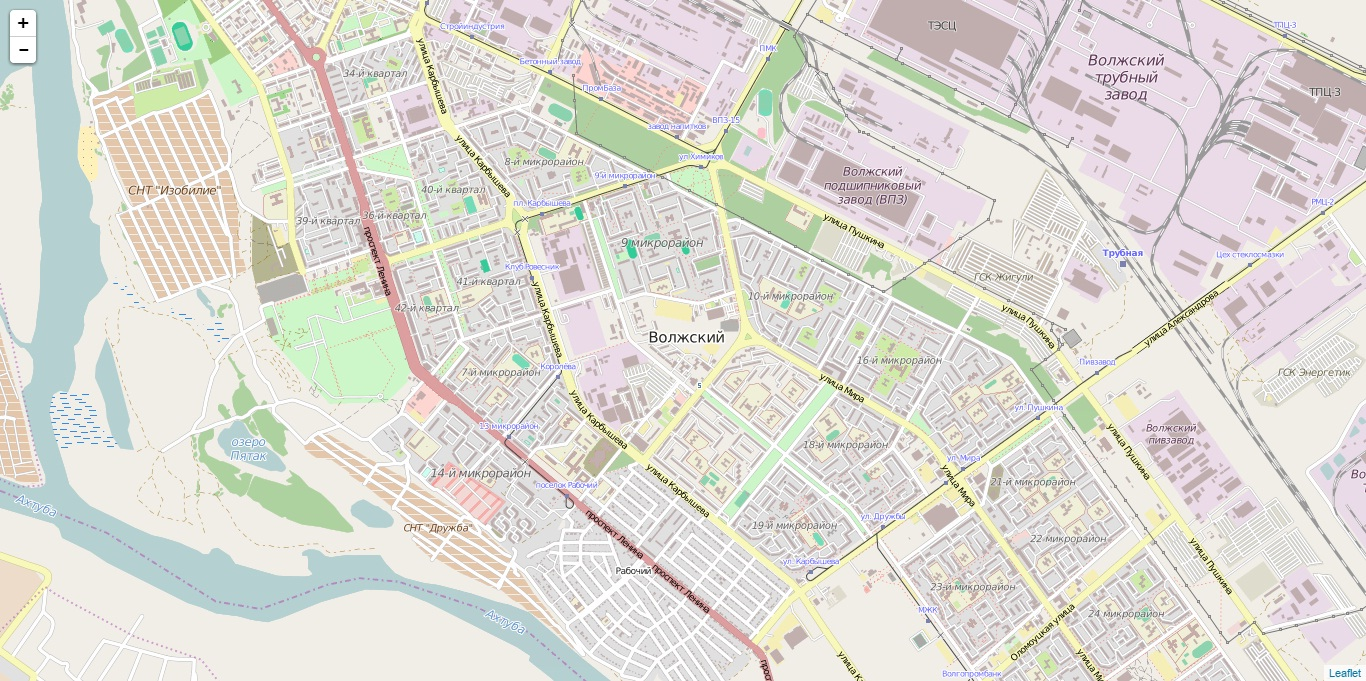
\includegraphics[width=.7\textwidth]{e1}
    \caption{Отображение карты}
\end{figure}

\subsubsection{Маркеры, круги и всплывающие сообщения}
Допустим, нам дан набор данных из 10 точек, который нужно отобразить на карте:
\lstinputlisting[language=js,firstline=14,lastline=23]{example/main.js}

Отобразить точку можно различными способами, здесь мы рассмотрим два 
основных: круг и маркер.

Обычный маркер создается командой \code{L.marker([широта, долгота])}. 
Создадим маркеры для всех точек:
\begin{lstlisting}[language=js]
    for (i in data) {
        L.marker(data[i]).addTo(map);
    }
\end{lstlisting}

Результат можно увидеть на рисунке~\ref{pic:e2}.

Для того, чтобы при нажатии на маркер всплывало сообщение с его координатами, 
привяжем к маркеру так называемый \emph{popup}:
\begin{lstlisting}[language=js]
    for (i in data) {
        marker = L.marker(data[i]).addTo(map);
        marker.bindPopup(data[i][0] + ‘, ‘ + data[i][1]);
    }
\end{lstlisting}
Или:
\begin{lstlisting}[language=js]
    for (i in data) {
        L.marker(data[i]).addTo(map).bindPopup(data[i][0] + ‘, ‘ + data[i][1]);
    }
\end{lstlisting}

\begin{figure}[h!]
    \center
    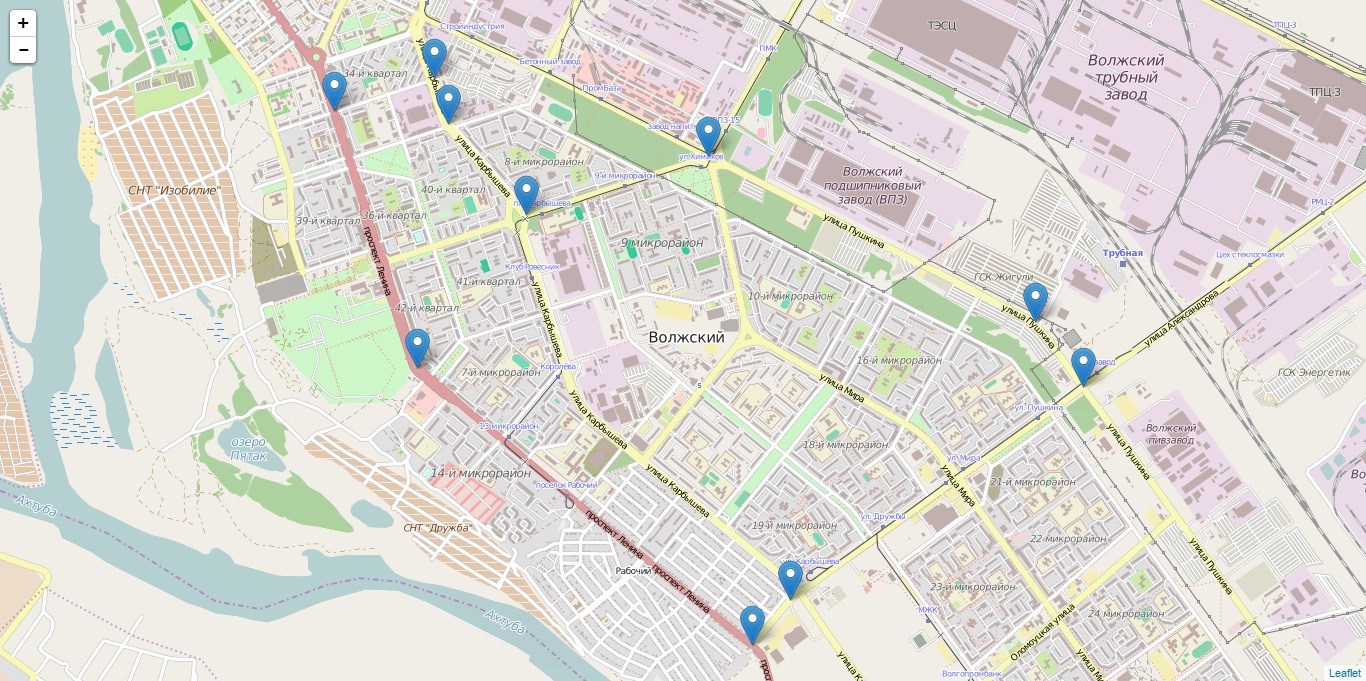
\includegraphics[width=.7\textwidth]{e2}
    \caption{Создание маркеров}
    \label{pic:e2}
\end{figure}

Команда \code{bindPopup(html\_text)} позволяет при нажатии на маркер отображать 
текст, оформленный с помощью html-тегов, записанный в переменной 
\code{html\_text}. Стандартно, на карте одновременно может отображаться не 
больше одного сообщения, поэтому при вызове нового сообщения старое 
автоматически закрывается. Таким образом, после нажатия на маркер получаем 
следующую картину: 
\begin{figure}[ht!]
    \center
    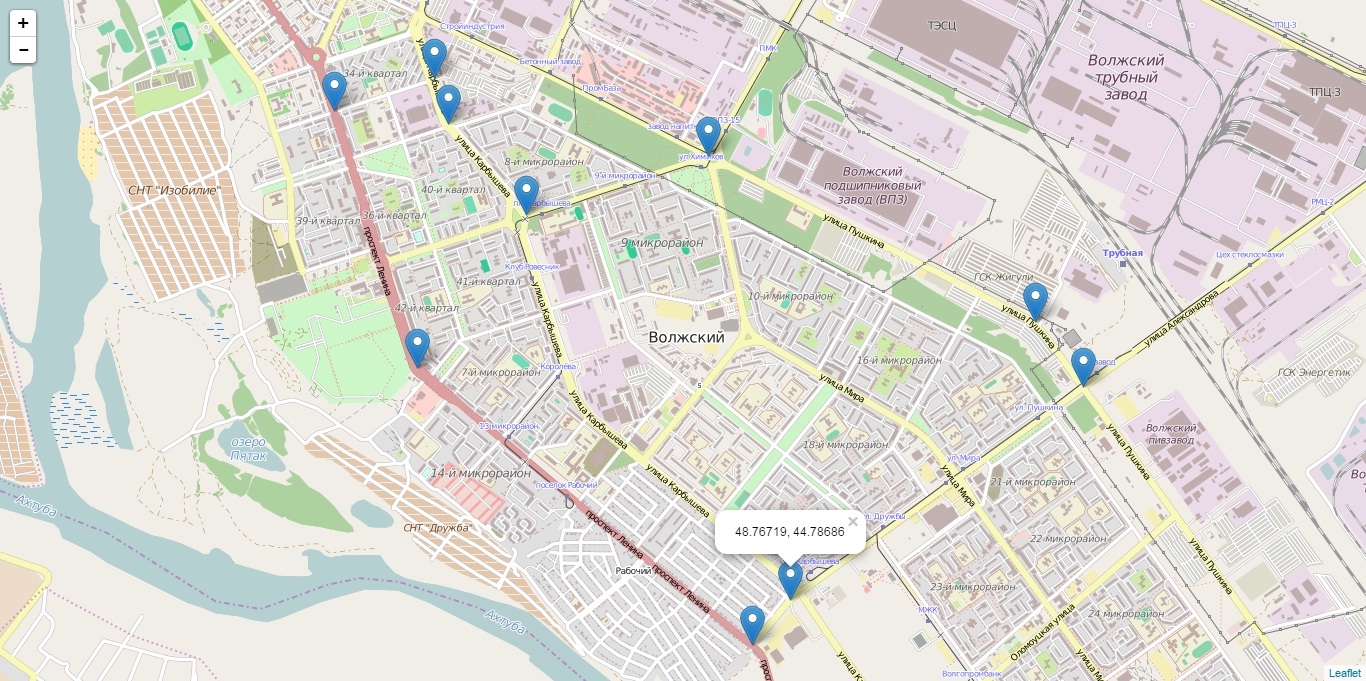
\includegraphics[width=.7\textwidth]{e3}
    \caption{Привязка сообщений к маркерам}
\end{figure}

Теперь вместо маркеров отобразим точки кругами. Для создания круга 
используется команда \code{L.circle([широта, долгота], радиус)}. Отобразим 
круги для всех точек:
\begin{lstlisting}[language=js]
    for (i in data) {
        L.circle(data[i], 50).addTo(map);
    }
\end{lstlisting}
Применяя уже знакомый метод \code{bindPopup}, привяжем сообщение с 
координатами на нажатие круга:
\begin{lstlisting}[language=js]
    for (i in data) {
        L.circle(data[i], 50).addTo(map).bindPopup(data[i][0] + ‘, ‘ + data[i][1]);
    }
\end{lstlisting}

Полученный результат:
\begin{figure}[ht!]
    \center
    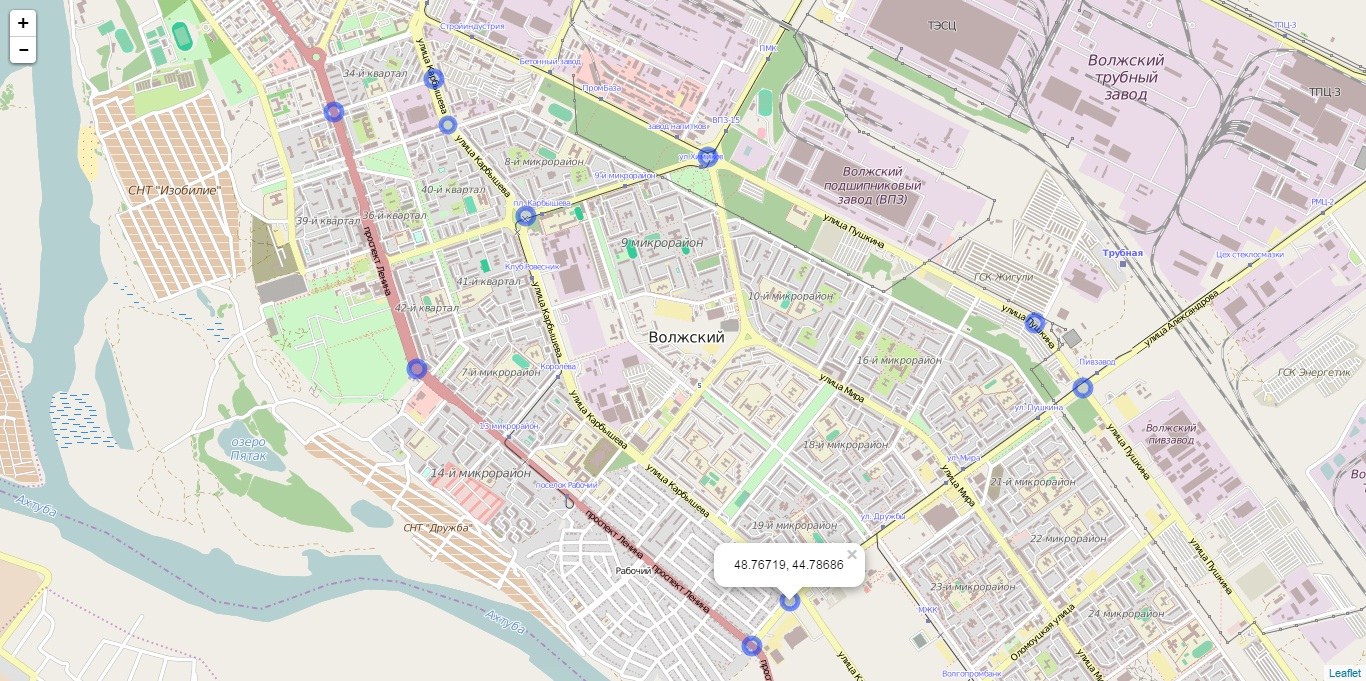
\includegraphics[width=.7\textwidth]{e4}
    \caption{Создание кругов}
    \label{pic:e4}
\end{figure}

Привяжем теперь всплывающее сообщение о координатах к нажатию на карту в 
любом месте. Для этого нам придется отлавливать событие клика и вызывать 
функцию отображения всплывающего сообщения.

Чтобы при нажатии левой кнопкой мыши на карту выполнялась функция 
\code{onClick} необходимо вызвать метод \code{on} карты \code{map}:
\lstinputlisting[language=js,firstline=3,lastline=3]{example/main.js}

Здесь \code{'click'} -- это название события. Теперь при клике на карту будет 
вызвана функция \code{onClick}, которой передадут так называемый 
\emph{event object} в качестве аргумента. В нашем случае это будет 
\emph{MouseEvent}.

Теперь напишем функцию вызова всплывающего сообщения. Для начала вне функции 
определим объект типа \code{L.popup}, который и будет являться нашим 
сообщением. В функции \code{onClick} мы тогда будем просто менять координаты 
вызова и текст сообщения.

\lstinputlisting[language=js,firstline=5,lastline=12]{example/main.js}

Разберем тело функции построчно. Первыми двумя строчками мы задаем 
переменным \code{lat} и \code{lng} некоторые значения. \code{e.latlng} -- это 
объект, содержащий в себе координаты точки, в нашем случае -- точки клика 
пользователя на карте; \code{e.latlng.lat} -- широта, \code{e.latlng.lng} -- 
долгота. Таким образом, переменные \code{lat} и \code{lng} хранят в себе 
координаты точки клика на карте с 5 знаками после запятой. Следующей строчкой 
мы задаем координаты нашего всплывающего сообщения методом \code{setLatLng}. 
Затем задаем \emph{контент} -- текст сообщения. Мы выводим координаты клика, 
причем полужирного начертания. Последней строчкой, как не трудно догадаться, 
мы показываем наше сообщение на карте.

Результат:
\begin{figure}[ht!]
    \center
    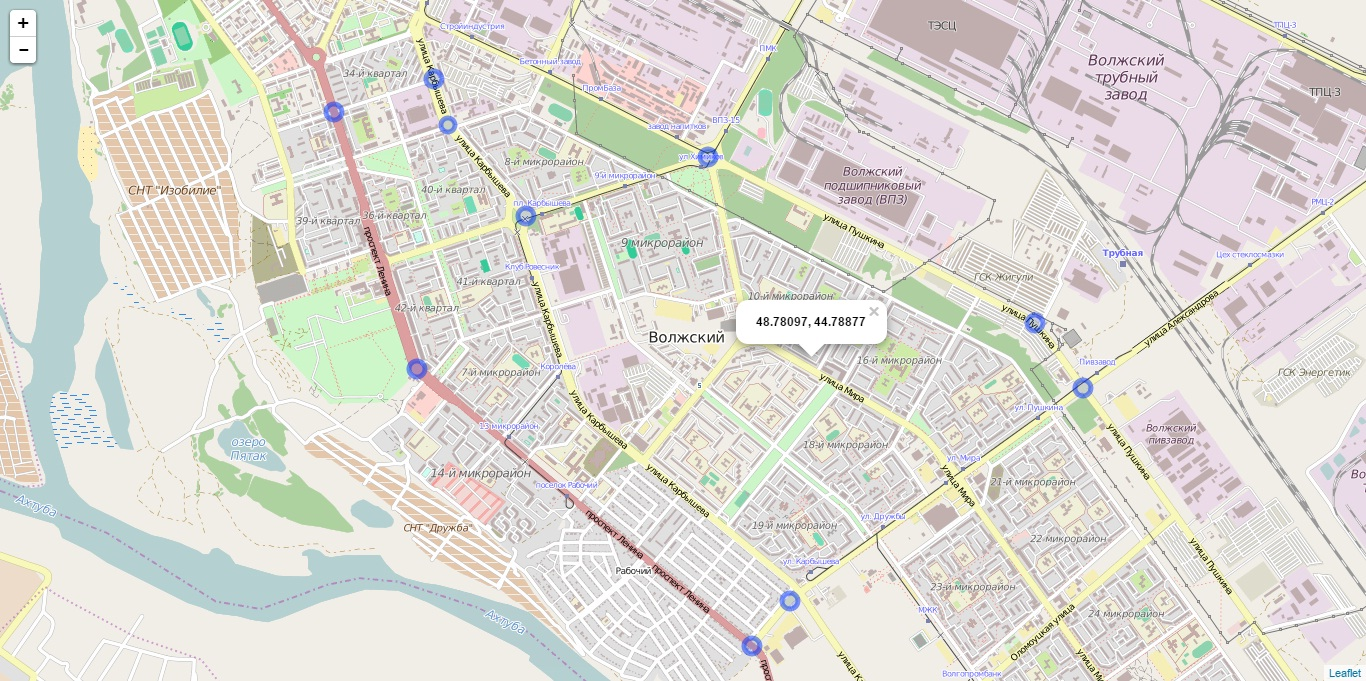
\includegraphics[width=.7\textwidth]{e5}
    \caption{Всплывающее сообщение при клике на карту}
    \label{pic:e5}
\end{figure}

\subsubsection{Ломаная и область}
При необходимости выделить область на карте или проложить маршрут используют 
объекты \emph{polygon} и \emph{polyline}.

Для создания ломаной по нашим точкам, необходимо сделать следующее:
\begin{lstlisting}[language=js]
    L.polyline(data).addTo(map);
\end{lstlisting}

Теперь у нас есть ломаная, соединяющая по порядку точки из нашего набора. 
Немного \emph{приукрасим} ее: изменим цвет и толщину. Для этого после набора 
данных \code{data} функции надо передать объект свойств ломаной; за цвет отвечает 
свойство \code{color}, за толщину -- \code{weight}:
\lstinputlisting[language=js,firstline=34,lastline=34]{example/main.js}

Таким же образом можно менять стиль кругов, изображающих наши точки:
\begin{lstlisting}[language=js]
    L.circle(data[i], 50, {color: ‘#f00’}).addTo(map);
\end{lstlisting}

После этого круги у нас будут красного цвета, а линия -- черная и узкая
(рис.~\ref{pic:e6}).
\begin{figure}[ht!]
    \center
    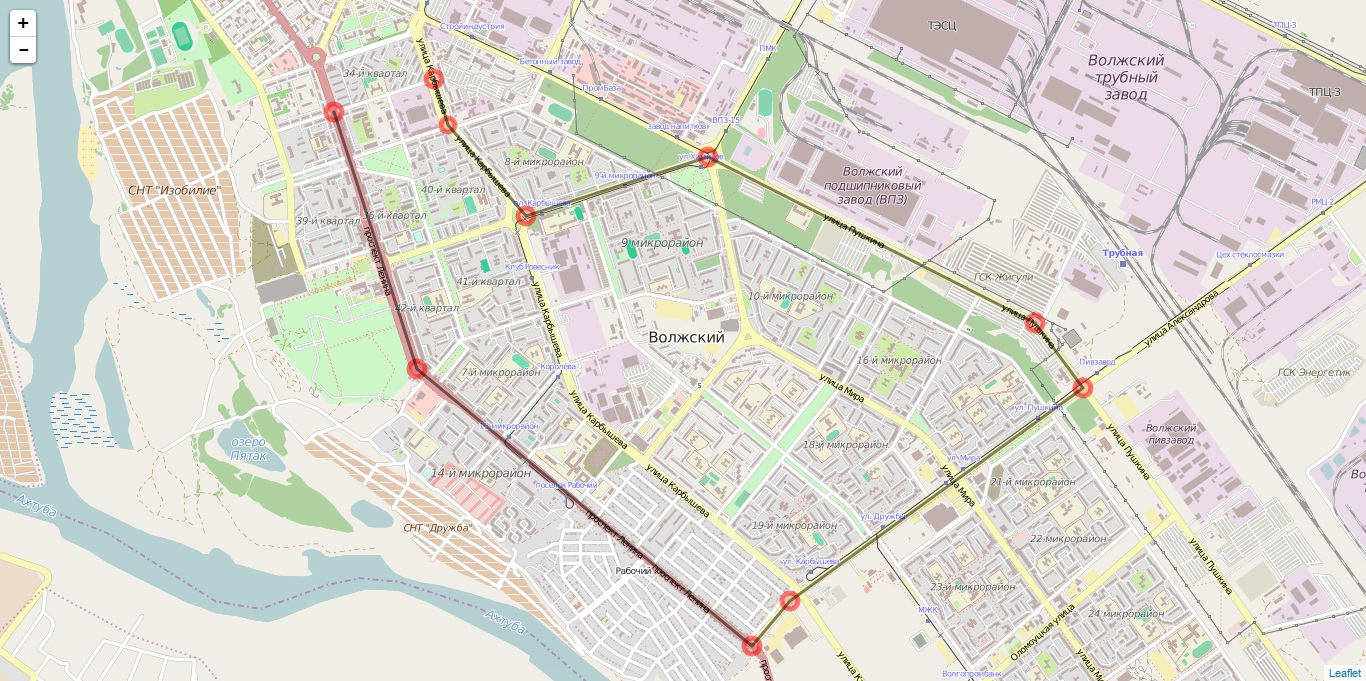
\includegraphics[width=.7\textwidth]{e6}
    \caption{Создание линии}
    \label{pic:e6}
\end{figure}

Для выделения области (полигона) необходимо создать объект \emph{polygon}:
\begin{lstlisting}[language=js]
    L.polygon(data, {color: 'green'}).addTo(map);
\end{lstlisting}
После этого область, задаваемая нашими точками, окрасится в зеленый цвет.
Если вместо нашего массива координат \code{data} передать массив массивов
точек \code{[data, data1, data2, \ldots]}, то перекрываемые области будут
вырезаться из полигона, а неперекрываемые -- добавляться.

Привяжем к нашему полигону какое-нибудь сообщение:
\lstinputlisting[language=js,firstline=36,lastline=37]{example/main.js}

Результат ожидаем:
\begin{figure}[ht!]
    \center
    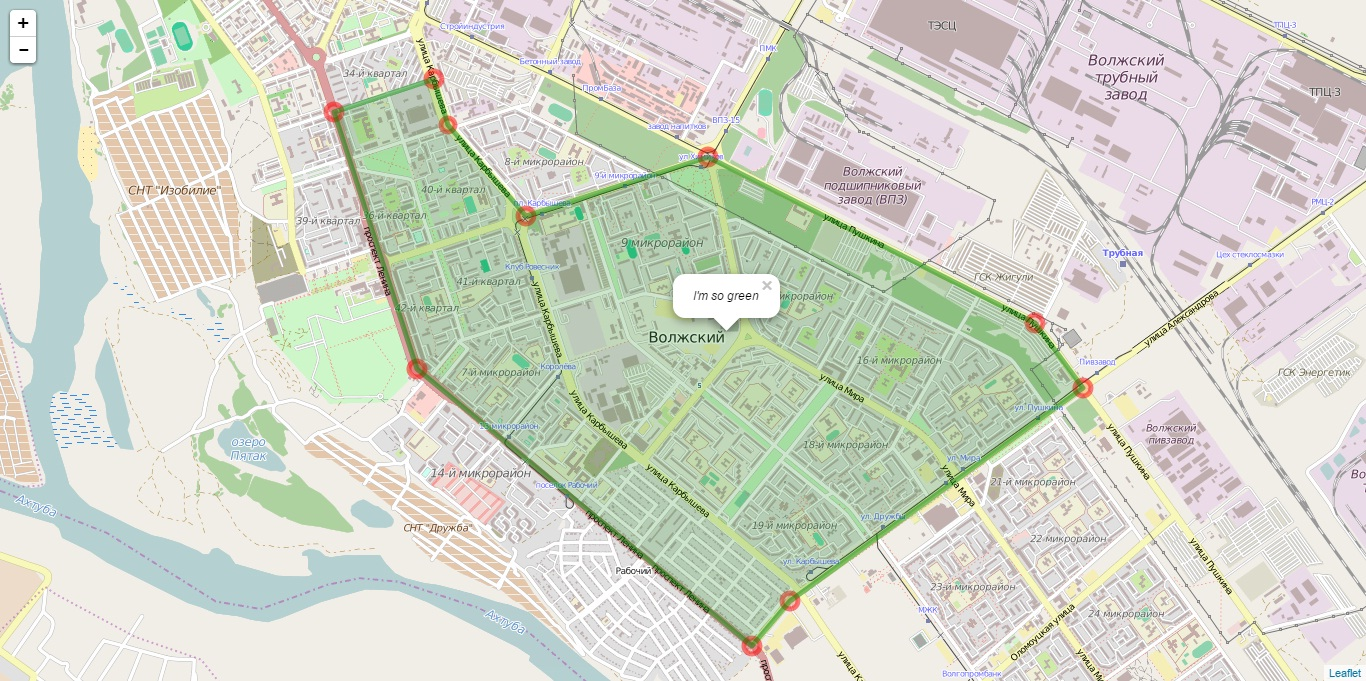
\includegraphics[width=.7\textwidth]{e7}
    \caption{Создание полигона}
    \label{pic:e7}
\end{figure}

Полный текст программы (логическая переменная \code{markers} отвечает за 
отображение точек в виде маркеров вместо кругов, логическая переменная 
\code{polyline} отвечает за отрисовку ломаной вместо полигона):
\lstinputlisting[language=js]{example/main.js}

\newpage

\section{Задания}
\begin{enumerate}
    \item Написать js-скрипт, который случайно расставляет точки на карте 
        в заданном диапазоне координат, задавая каждой точке уникальный 
        6-значный hex-идентификатор. Каждую точку отобразить на карте 
        кружком, цвет которого является значением идентификатора.
    \item Написать функцию рисования фигуры:
    \begin{itemize}
        \item треугольник,
        \item звезда,
        \item ломаная,
        \item <<бублик>>, то есть многоугольник с вырезанной областью внутри.
    \end{itemize}
    Для ломаной и внешней границы многоугольника используйте координаты точек,
    полученные в 1-ом задании.
    \item Изобразить точки из 1-го задания маркерами, по нажатию на который 
        выводится сообщение, содержащее идентификатор точки и ее координаты.
\end{enumerate}

\newpage

\section{Контрольные вопросы}
\begin{enumerate}
    \item Назовите базовые типы географических данных в OpenStreetMap. 
        Кратко расскажите о них. Для чего они нужны?
    \item Чем или почему проект OpenStreetMap лучше многих других?
    \item Зачем нужен тип данных отношение (\emph{relation})?
    \item Зачем нужно теггирование объектов? Для чего оно используется?
    \item Преимущества и недостатки библиотеки Leaflet.
    % можно написать еще
\end{enumerate}

\newpage

\section{Ссылки и примечания}
\begin{thebibliography}{10}
    \bibitem{habrahabr01} Зачем миру нужен OpenStreetMap 
        \url{http://habrahabr.ru/post/217291/}
    \bibitem{habrahabr02} Структура данных проекта OpenStreetMap, заглянем под 
        юбку сервису \url{http://habrahabr.ru/post/146503/}
    \bibitem{waze} Приложение дорожной навигации \url{https://www.waze.com/}
    \bibitem{navteq} Ведущий в мире производитель цифровых карт и других 
        данных для геоинформационных систем \url{www.navteq.com}
    \bibitem{tomtom} Нидерландская компания, поставщик устройств для 
        автомобильной и персональной GPS-навигации \url{www.tomtom.com}
    \bibitem{teleatlas} Глобальным поставщик навигационных карт для 
        автомобильных навигационных систем, геоинформационных и 
        локально-информационных систем \url{www.tomtom.com}
    \bibitem{four4} Cоциальная сеть с функцией геопозиционирования, 
        предназначенная в основном для работы с мобильными устройствами.
        \url{https://foursquare.com/}
    \bibitem{ingress} Многопользовательская онлайн-игра, созданная 
        Niantic Labs в Google для Android- и iOS-устройств 
        \url{https://www.ingress.com/}
    \bibitem{floss} The Free-Libre / Open Source Software (FLOSS) License\\
        \url{http://www.dwheeler.com/essays/floss-license-slide.html}
    \bibitem{osmwiki} \url{https://ru.wikipedia.org/wiki/OpenStreetMap}
    \bibitem{osmformat} \url{http://wiki.openstreetmap.org/wiki/RU:Map_Features}
    \bibitem{leaflet} Open-Source библиотека предназначенная для отображения 
        карт на веб-сайтах \url{http://leafletjs.com/}
    \bibitem{openlayers} Библиотека с открытым исходным кодом, написанная на 
        JavaScript, предназначенная для создания карт 
        \url{http://openlayers.org/}
    \bibitem{projection} Проекция Меркатора 
        \href{https://ru.wikipedia.org/wiki/%D0%9F%D1%80%D0%BE%D0%B5%D0%BA%D1%86%D0%B8%D1%8F_%D0%9C%D0%B5%D1%80%D0%BA%D0%B0%D1%82%D0%BE%D1%80%D0%B0}
        {https://ru.wikipedia.org/wiki/Проекция\_Меркатора}
\end{thebibliography}
